\chapter{Alberi di Decisione}
\begin{flushright}\small\textit{Lezione 7 -- 30/03/2026 -- G\'eron, Cap.\ 6}\end{flushright}

\section{Introduzione}

Gli \textbf{Alberi di Decisione} (Decision Trees) sono algoritmi di Machine Learning supervisionato estremamente intuitivi: a differenza di altri modelli, non cercano equazioni matematiche complesse, ma si basano su una serie di \textbf{domande a cascata} (\texttt{if/else}). Sono algoritmi versatili, utilizzabili per:

\begin{itemize}
    \item \textbf{Classificazione} (\texttt{DecisionTreeClassifier}): classificare iris, riconoscere cifre, filtrare spam.
    \item \textbf{Regressione} (\texttt{DecisionTreeRegressor}): stimare prezzi, prevedere valori continui.
    \item Predizioni \textbf{multioutput}: più output contemporaneamente.
\end{itemize}

Richiedono pochissimo preprocessing: nessun \emph{feature scaling} o \emph{centering}. Sono la componente fondamentale delle \textbf{Random Forest} e di altri ensemble, tra i modelli più potenti disponibili oggi su dati tabulari.

Fanno parte della \textbf{xAI (Explainable AI)}:
\begin{itemize}
    \item \textbf{White Box} (scatola trasparente): l'analista capisce perfettamente perché il modello ha preso una decisione -- basta leggere la sequenza di \texttt{if/else}.
    \item \textbf{Black Box} (scatola nera): algoritmi come le reti neurali profonde. Funzionano benissimo, ma la logica matematica interna è incomprensibile all'uomo.
\end{itemize}

L'interpretabilità è cruciale in ambiti regolamentati: \emph{credit scoring}, sanità, sistemi di giustizia, GDPR Art.\ 22 (diritto a non essere soggetti a decisioni automatizzate non spiegate).

\section{Come funziona -- l'esempio Iris}

Usiamo il dataset Iris con solo 2 feature: \textbf{lunghezza} e \textbf{larghezza del petalo}. L'albero impara a classificare le tre specie (Setosa, Versicolor, Virginica) tramite soglie sulle feature.


\begin{center}
\begin{tikzpicture}[font=\small,
    inode/.style={draw=MidnightBlue, very thick, rounded corners=5pt,
                  fill=blue!8, text width=5.2cm, align=center, minimum height=1.1cm},
    leaf/.style={draw=OliveGreen, very thick, rounded corners=5pt,
                 fill=green!8, text width=3.6cm, align=center, minimum height=1.1cm}
]
\node[inode] (root) at (0,0)
    {\textbf{Nodo radice}\\petal length $\leq 2{,}45$\,cm\\samples = 150, \quad$[50,50,50]$\\Gini $= 0{,}667$};

\node[leaf] (l1) at (-4.5, -2.6)
    {\textbf{Foglia -- Setosa}\\samples = 50\\$[50,0,0]$\\Gini $= 0$};

\node[inode] (n2) at (3.0, -2.6)
    {\textbf{Nodo interno}\\petal width $\leq 1{,}75$\,cm\\samples = 100, \quad$[0,50,50]$\\Gini $= 0{,}5$};

\node[leaf] (l2) at (0.5, -5.2)
    {\textbf{Foglia -- Versicolor}\\samples = 54\\$[0,49,5]$\\Gini $= 0{,}168$};

\node[leaf] (l3) at (5.5, -5.2)
    {\textbf{Foglia -- Virginica}\\samples = 46\\$[0,1,45]$\\Gini $= 0{,}042$};

\draw[-{Stealth[length=3mm]}, thick, OliveGreen]
    (root.south west) -- (l1.north)
    node[midway, above, sloped, font=\scriptsize\bfseries, OliveGreen] {Sì};
\draw[-{Stealth[length=3mm]}, thick, BrickRed]
    (root.south east) -- (n2.north)
    node[midway, above, sloped, font=\scriptsize\bfseries, BrickRed] {No};
\draw[-{Stealth[length=3mm]}, thick, OliveGreen]
    (n2.south west) -- (l2.north)
    node[midway, above, sloped, font=\scriptsize\bfseries, OliveGreen] {Sì};
\draw[-{Stealth[length=3mm]}, thick, BrickRed]
    (n2.south east) -- (l3.north)
    node[midway, above, sloped, font=\scriptsize\bfseries, BrickRed] {No};
\end{tikzpicture}
\end{center}

\textbf{Come ragiona l'albero}: si parte sempre dal nodo radice e si scende lungo i rami seguendo il valore della feature.

\begin{enumerate}
    \item \textbf{Nodo radice}: ``La lunghezza del petalo è $\leq 2{,}45$ cm?''
    \begin{itemize}
        \item \textbf{Sì} $\to$ 50 fiori, tutti Setosa $[50,0,0]$ $\to$ nodo puro, \textbf{foglia}.
        \item \textbf{No} $\to$ 100 fiori misti $[0,50,50]$ $\to$ nodo impuro, serve un'altra domanda.
    \end{itemize}
    \item \textbf{Nodo interno}: ``La larghezza del petalo è $\leq 1{,}75$ cm?''
    \begin{itemize}
        \item \textbf{Sì} $\to$ 54 fiori, di cui 49 Versicolor $[0,49,5]$ $\to$ foglia, classe predetta: Versicolor.
        \item \textbf{No} $\to$ 46 fiori, di cui 45 Virginica $[0,1,45]$ $\to$ foglia, classe predetta: Virginica.
    \end{itemize}
\end{enumerate}

Alla foglia, la \textbf{probabilità stimata} è il rapporto istanze-classe/totale: $49/54 \approx 90{,}7\%$ per Versicolor. La classe predetta è quella con la probabilità più alta.

\begin{notebox}[Spesso i dataset hanno migliaia di attributi]
L'albero di decisione ignora automaticamente le feature inutili e seleziona solo quelle davvero discriminanti. Nel caso Iris con 4 feature, l'algoritmo sceglie autonomamente di usare solo lunghezza e larghezza del petalo, ignorando le misure del sepalo.
\end{notebox}

\subsection{I confini di decisione}

Riportando l'albero su un piano cartesiano, i \textbf{decision boundary} sono sempre \emph{linee rette orizzontali e verticali} -- mai curve o oblique. La linea verticale spessa (depth 0) separa Setosa da tutto il resto. La linea orizzontale tratteggiata (depth 1) separa Versicolor da Virginica. Aumentando \texttt{max\_depth} si aggiungono ulteriori linee ortogonali -- ma si rischia overfitting.


\begin{center}
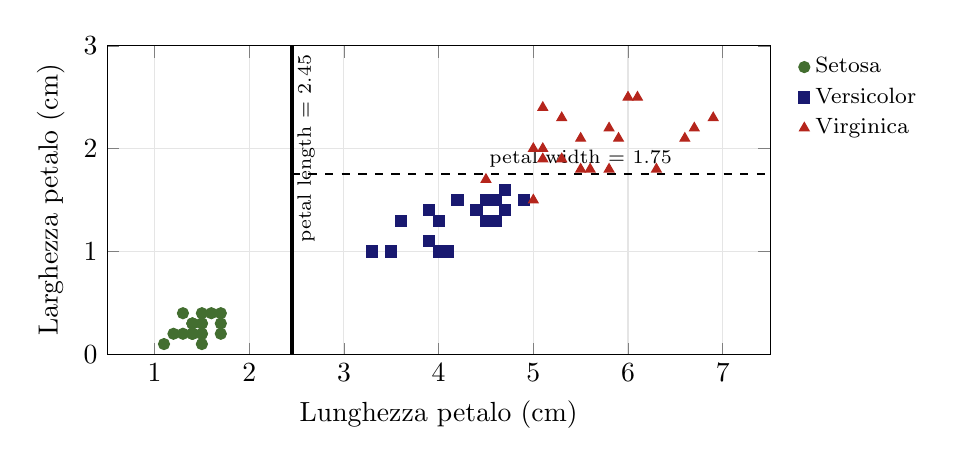
\begin{tikzpicture}
\begin{axis}[
    width=10cm, height=5.5cm,
    xlabel={Lunghezza petalo (cm)},
    ylabel={Larghezza petalo (cm)},
    xmin=0.5, xmax=7.5, ymin=0, ymax=3.0,
    grid=major, grid style={gray!20},
    legend pos=outer north east,
    legend style={font=\footnotesize, cells={anchor=west},
                  legend columns=1, draw=none}
]
\addplot[only marks, mark=*, mark size=2pt, OliveGreen!80!black]
    coordinates {(1.4,0.2)(1.3,0.2)(1.5,0.2)(1.7,0.4)(1.4,0.3)(1.5,0.2)
                 (1.4,0.2)(1.5,0.1)(1.5,0.3)(1.4,0.2)(1.6,0.4)(1.4,0.3)
                 (1.1,0.1)(1.2,0.2)(1.5,0.4)(1.3,0.4)(1.4,0.3)(1.7,0.3)
                 (1.5,0.3)(1.7,0.2)};
\addlegendentry{Setosa}
\addplot[only marks, mark=square*, mark size=2pt, MidnightBlue]
    coordinates {(4.7,1.4)(4.5,1.5)(4.9,1.5)(4.0,1.3)(4.6,1.5)(4.5,1.3)
                 (4.7,1.6)(3.3,1.0)(4.6,1.3)(3.9,1.4)(3.5,1.0)(4.2,1.5)
                 (4.0,1.0)(4.7,1.4)(3.6,1.3)(4.4,1.4)(4.5,1.5)(4.1,1.0)
                 (4.5,1.5)(3.9,1.1)};
\addlegendentry{Versicolor}
\addplot[only marks, mark=triangle*, mark size=2pt, BrickRed]
    coordinates {(6.0,2.5)(5.1,1.9)(5.9,2.1)(5.6,1.8)(5.8,2.2)(6.6,2.1)
                 (4.5,1.7)(6.3,1.8)(5.8,1.8)(6.1,2.5)(5.1,2.0)(5.3,1.9)
                 (5.5,2.1)(5.0,2.0)(5.1,2.4)(5.3,2.3)(5.5,1.8)(6.7,2.2)
                 (6.9,2.3)(5.0,1.5)};
\addlegendentry{Virginica}
\addplot[very thick, black] coordinates {(2.45,0)(2.45,3.0)};
\node[font=\scriptsize, rotate=90] at (axis cs:2.6, 2.0) {petal length = 2.45};
\addplot[thick, black, dashed] coordinates {(2.45,1.75)(7.5,1.75)};
\node[font=\scriptsize] at (axis cs:5.5, 1.9) {petal width = 1.75};
\end{axis}
\end{tikzpicture}
\end{center}


\section{Metriche di impurità}
Come decide l'algoritmo qual è la \textbf{domanda migliore} da fare a ogni nodo? Cerca la domanda (feature + soglia) che divide i dati nei gruppi più ``puri'' possibile. Due metriche:

\subsection{Indice di Gini}

\begin{equation}
\boxed{G_i = 1 - \sum_{k=1}^{n} p_{i,k}^2}
\end{equation}

dove $p_{i,k}$ è la proporzione della classe $k$ nel nodo $i$.

\begin{itemize}
    \item Nodo \textbf{puro} (tutti della stessa classe): $G = 0$.
    \item Nodo completamente \textbf{misto} ($K$ classi equiprobabili): $G = 1 - 1/K$. Per 2 classi: massimo $G = 0{,}5$.
\end{itemize}

\begin{exbox}[Calcolo di Gini per tutti i nodi dell'albero Iris]
\textbf{Nodo radice} $[50, 50, 50]$, totale $= 150$:
\[
G = 1 - \left(\frac{50}{150}\right)^2 - \left(\frac{50}{150}\right)^2 - \left(\frac{50}{150}\right)^2
= 1 - 3 \times \frac{1}{9} = 1 - \frac{1}{3} \approx 0{,}667
\]

\textbf{Nodo Setosa} $[50, 0, 0]$: \quad $G = 1 - 1^2 - 0 - 0 = 0$ (puro)

\textbf{Nodo depth-1 dx} $[0, 50, 50]$:
\[
G = 1 - 0 - \left(\frac{50}{100}\right)^2 - \left(\frac{50}{100}\right)^2 = 1 - 0{,}25 - 0{,}25 = 0{,}5
\]

\textbf{Nodo Versicolor} $[0, 49, 5]$, totale $= 54$:
\[
G = 1 - 0 - \left(\frac{49}{54}\right)^2 - \left(\frac{5}{54}\right)^2
= 1 - 0{,}823 - 0{,}009 \approx 0{,}168
\]

\textbf{Nodo Virginica} $[0, 1, 45]$, totale $= 46$:
\[
G = 1 - 0 - \left(\frac{1}{46}\right)^2 - \left(\frac{45}{46}\right)^2
\approx 1 - 0{,}000 - 0{,}958 = 0{,}042
\]
\end{exbox}

\subsection{Entropia di Shannon}

\begin{equation}
H_i = -\sum_{k=1}^{n} p_{i,k} \cdot \log_2 p_{i,k}
\end{equation}

Il concetto di entropia viene dalla termodinamica (misura il disordine) e dalla teoria dell'informazione di Shannon (misura l'imprevedibilità). Nodo puro ($p=1$), allora $\log_2(1) = 0 e quindi anche l'entropia \Rightarrow H = 0$.

\begin{exbox}[Entropia del nodo Versicolor {$[0,49,5]$}]
\[
H = -\frac{49}{54}\log_2\!\frac{49}{54} - \frac{5}{54}\log_2\!\frac{5}{54}
\approx -(0{,}907 \times (-0{,}141)) - (0{,}093 \times (-3{,}426))
\approx 0{,}445
\]
\end{exbox}

\begin{notebox}[Gini vs Entropia: quale scegliere?]
In pratica producono alberi molto simili e con prestazioni analoghe. Differenze:
\begin{itemize}
    \item \textbf{Gini} (default Scikit-learn): leggermente più veloce (nessun calcolo di logaritmo); tende a isolare la classe più frequente in un ramo.
    \item \textbf{Entropia}: produce alberi leggermente più bilanciati.
\end{itemize}
Gini è un buon punto di partenza. Il criterio si imposta con \texttt{criterion="entropy"} in Scikit-learn.
\end{notebox}

\section{L'algoritmo CART}

Scikit-learn usa l'algoritmo \textbf{CART} (Classification and Regression Trees, Breiman 1984) per costruire alberi binari (ogni nodo ha esattamente 2 figli).

Ad ogni passo, CART cerca la coppia (feature $k$, soglia $t_k$) che minimizza la funzione di costo:

\begin{equation}
\boxed{J(k,\, t_k) = \frac{m_\text{left}}{m} \cdot G_\text{left} + \frac{m_\text{right}}{m} \cdot G_\text{right}}
\end{equation}

È una \textbf{media pesata} dell'impurità dei due nodi figli, dove il peso è la proporzione di istanze. Il processo è ricorsivo: ogni sottoinsieme viene ulteriormente diviso, finché non si raggiunge un criterio di arresto (profondità massima, minimo campioni, ecc.).

\subsection{CART è un algoritmo greedy}

\begin{defbox}[Approccio Greedy]
CART prende la decisione \textbf{localmente migliore} in ogni nodo, senza guardare avanti di più livelli. Non garantisce di trovare l'albero ottimale globale.

Trovare l'albero perfetto è un problema \textbf{NP-Completo} -- costo esponenziale $O(e^m)$, intrattabile anche per dataset piccoli. Ci si accontenta dell'ottimo locale trovato dall'approccio greedy.
\end{defbox}

\begin{exbox}[Confronto con Dijkstra]
Dijkstra (algoritmo per i percorsi minimi sui grafi) è anch'esso greedy: ``qual è la città inesplorata più vicina? Ci vado!''. La differenza fondamentale: Dijkstra \textbf{garantisce} l'ottimo globale (a patto che non ci siano archi con peso negativo). CART \textbf{non} garantisce l'ottimo globale -- due alberi addestrati sullo stesso dataset con semi diversi possono risultare significativamente diversi.
\end{exbox}

\subsection{Costo computazionale}

\begin{itemize}
    \item \textbf{Inferenza} (previsione): scendere dall'albero radice a una foglia. Per un albero bilanciato: $O(\log_2 m)$. Velocissimo, indipendente dal numero di feature.
    \item \textbf{Training}: a ogni nodo si confrontano tutte le $n$ feature su tutte le $m$ istanze. Complessità: $O(n \cdot m \log_2 m)$. Scalabile a dataset ragionevolmente grandi.
\end{itemize}

\begin{exbox}[Esempio pratico]
Se il training con $m = 10^6$ istanze richiede 1 ora, con $m = 10^7$ richiederà circa:
\[
\frac{10^7 \cdot \log_2(10^7)}{10^6 \cdot \log_2(10^6)} \approx \frac{10 \times 23{,}25}{19{,}93} \approx 11{,}7 \text{ ore}
\]
(non 10 ore: il $\log$ cresce leggermente con $m$).
\end{exbox}

\section{Regressione con gli alberi di decisione}

\texttt{DecisionTreeRegressor} funziona con la stessa struttura: nodi interni con test su feature, foglie con valori continui. La differenza è nella \textbf{funzione di costo}: invece di minimizzare Gini, si minimizza l'MSE ponderato.

\begin{equation}
J(k, t_k) = \frac{m_\text{left}}{m} \cdot MSE_\text{left} + \frac{m_\text{right}}{m} \cdot MSE_\text{right}
\end{equation}

dove:
\[
\bar{y}_\text{node} = \frac{1}{m_\text{node}} \sum_{i \in \text{node}} y_i
\qquad
MSE_\text{node} = \frac{1}{m_\text{node}} \sum_{i \in \text{node}} (y_i - \bar{y}_\text{node})^2
\]

La previsione in ogni foglia è la \textbf{media} dei valori target delle istanze che vi arrivano. Il risultato è una funzione a scalini -- più è profondo l'albero, più i gradini sono piccoli.

\begin{center}
\begin{tikzpicture}
\begin{groupplot}[
    group style={group size=2 by 1, horizontal sep=1.5cm},
    width=6cm, height=4.5cm,
    xlabel={$x$}, ylabel={$y$},
    xmin=-0.6, xmax=0.6, ymin=-0.05, ymax=0.35,
    grid=major, grid style={gray!20},
    title style={font=\small\bfseries}
]
\nextgroupplot[title={Regressione -- depth $= 2$}]
\addplot[only marks, mark=*, mark size=1.2pt, MidnightBlue!60]
    coordinates {
        (-0.5,0.25)(-0.45,0.20)(-0.4,0.16)(-0.35,0.12)(-0.3,0.09)
        (-0.25,0.06)(-0.2,0.04)(-0.15,0.023)(-0.1,0.012)(-0.05,0.003)
        (0,0.002)(0.05,0.003)(0.1,0.011)(0.15,0.022)(0.2,0.04)
        (0.25,0.065)(0.3,0.092)(0.35,0.122)(0.4,0.163)(0.45,0.205)(0.5,0.25)
    };
\addplot[very thick, BrickRed, const plot mark left]
    coordinates {(-0.6,0.175)(-0.3,0.175)(-0.3,0.039)(0,0.039)
                 (0,0.039)(0.3,0.039)(0.3,0.175)(0.6,0.175)};
\nextgroupplot[title={Regressione -- depth $= 3$}]
\addplot[only marks, mark=*, mark size=1.2pt, MidnightBlue!60]
    coordinates {
        (-0.5,0.25)(-0.45,0.20)(-0.4,0.16)(-0.35,0.12)(-0.3,0.09)
        (-0.25,0.06)(-0.2,0.04)(-0.15,0.023)(-0.1,0.012)(-0.05,0.003)
        (0,0.002)(0.05,0.003)(0.1,0.011)(0.15,0.022)(0.2,0.04)
        (0.25,0.065)(0.3,0.092)(0.35,0.122)(0.4,0.163)(0.45,0.205)(0.5,0.25)
    };
\addplot[very thick, OliveGreen, const plot mark left]
    coordinates {(-0.6,0.22)(-0.45,0.22)(-0.45,0.115)(-0.3,0.115)
                 (-0.3,0.052)(-0.15,0.052)(-0.15,0.012)(0,0.012)
                 (0,0.012)(0.15,0.012)(0.15,0.053)(0.3,0.053)
                 (0.3,0.116)(0.45,0.116)(0.45,0.223)(0.6,0.223)};
\end{groupplot}
\end{tikzpicture}
\end{center}

Anche la regressione è soggetta a overfitting: senza limiti, l'albero crea una foglia per ogni punto del training set, con previsioni perfette ma generalizzazione pessima. La regolarizzazione (es.\ \texttt{min\_samples\_leaf=10}) risolve il problema.

\section{Overfitting e regolarizzazione}

I decision tree sono modelli \textbf{non parametrici}: il numero di parametri non è fissato prima del training, ma cresce con i dati. Senza vincoli, l'albero cresce finché ogni foglia è pura al 100\% -- overfitting garantito.

\begin{exbox}[Effetto della regolarizzazione -- dataset Moons]
L'albero non regolarizzato produce confini di decisione estremamente irregolari e memorizza il rumore. L'albero con \texttt{min\_samples\_leaf=5} generalizza meglio nonostante un training accuracy leggermente inferiore.
\end{exbox}

Un approccio alternativo è il \textbf{pruning} (potatura): si fa crescere l'albero senza limiti, poi si rimuovono i nodi non significativi usando test statistici (es.\ test $\chi^2$). Se il miglioramento di purezza non è statisticamente significativo (p-value $> 5\%$), il nodo è eliminato.

\section{Sensibilità all'orientamento degli assi}

I confini di decisione sono \textbf{sempre perpendicolari agli assi delle feature}. Questo rende gli alberi sensibili all'orientamento dei dati: una semplice rotazione del dataset può trasformare un problema banale in uno che richiede molti più split.

\begin{center}
\begin{tikzpicture}
\begin{groupplot}[
    group style={group size=2 by 1, horizontal sep=2.0cm},
    width=5.5cm, height=5.0cm,
    xmin=-2, xmax=2, ymin=-2, ymax=2,
    xtick=\empty, ytick=\empty,
    axis equal,
    grid=none,
    title style={font=\small\bfseries}
]
\nextgroupplot[title={Dati originali -- facile}]
\addplot[only marks, mark=*, mark size=2pt, MidnightBlue]
    coordinates {(-1.5,0.5)(-1,1)(-0.5,1.5)(0,1.2)(-1.2,1.5)(-0.8,0.8)
                 (-1.6,0.2)(-0.3,0.6)(-1.1,0.3)(-0.6,1.0)};
\addplot[only marks, mark=square*, mark size=2pt, BrickRed]
    coordinates {(0.5,-0.5)(1,-1)(1.5,-0.5)(0.8,-1.2)(0.3,-0.8)
                 (1.2,-0.3)(0.6,-1.5)(1.5,-1.2)(0.2,-1.1)(1.0,-0.6)};
\addplot[very thick, OliveGreen] coordinates {(0,-2)(0,2)};
\nextgroupplot[title={Dati ruotati di 45° -- difficile}]
\addplot[only marks, mark=*, mark size=2pt, MidnightBlue]
    coordinates {(-1.4,0.1)(-1.4,0.7)(-1.4,1.4)(-0.8,0.8)(-1.2,1.2)
                 (-1.1,0.2)(-1.6,-0.4)(-0.6,0.6)(-1.0,-0.1)(-0.9,0.3)};
\addplot[only marks, mark=square*, mark size=2pt, BrickRed]
    coordinates {(0.7,-0.8)(1.4,-1.4)(1.4,-0.7)(1.0,-1.5)(0.7,-0.4)
                 (1.1,-0.8)(1.5,-0.4)(1.5,-1.4)(0.5,-0.8)(1.2,-0.9)};
\addplot[very thick, OliveGreen] coordinates {(-2,0.6)(-0.6,-0.6)(0.6,0.6)(2,-0.6)};
\end{groupplot}
\end{tikzpicture}
\end{center}

A sinistra, un solo taglio verticale separa perfettamente le due classi. A destra, dopo una rotazione di 45°, il confine naturale è diagonale ma l'albero può usare solo linee ortogonali -- servono molti più split, con rischio di overfitting.

\textbf{Soluzione}: pre-processare i dati con \textbf{StandardScaler + PCA} per ruotare e decorrelare le feature prima di addestrare l'albero.

\section{Alta varianza e Random Forest}

Gli alberi di decisione sono modelli ad \textbf{alta varianza}: piccole modifiche nei dati di training o un seed diverso possono produrre alberi strutturalmente molto diversi. L'algoritmo di training di Scikit-learn è stocastico (seleziona casualmente le feature da valutare a ogni nodo) -- anche riaddestrando sugli stessi dati si ottiene un albero differente.

Questa alta varianza sembra un difetto, ma negli \textbf{ensemble} diventa un punto di forza:

\begin{defbox}[Random Forest]
Una \textbf{Random Forest} è un ensemble di alberi di decisione, ciascuno addestrato su:
\begin{itemize}
    \item Un sottoinsieme casuale delle \textbf{istanze} (bootstrap sampling -- \emph{bagging}).
    \item Un sottoinsieme casuale delle \textbf{feature} a ogni split.
\end{itemize}
Le previsioni vengono combinate per \textbf{voto di maggioranza} (classificazione) o \textbf{media} (regressione). Mediando su tanti alberi diversi, la varianza si riduce drasticamente senza aumentare il bias -- le foreste generalizzano molto meglio dei singoli alberi.
\end{defbox}

\begin{exbox}[Dal singolo albero alla foresta -- costruzione manuale]
\begin{enumerate}
    \item Generare 1\,000 sottoinsiemi del training set, ciascuno con 100 istanze casuali.
    \item Addestrare un \texttt{DecisionTreeClassifier} su ciascun sottoinsieme.
    \item Per ogni istanza del test set, raccogliere le 1\,000 previsioni e tenere quella di maggioranza (\texttt{scipy.stats.mode}).
    \item Risultato: accuratezza leggermente superiore al singolo albero addestrato sull'intero training set.
\end{enumerate}
Questo è esattamente ciò che fa \texttt{RandomForestClassifier} in modo automatico ed efficiente.
\end{exbox}

Random Forest e \textbf{Gradient Boosting} (XGBoost, LightGBM, CatBoost) -- che addesstrano alberi in sequenza correggendo gli errori dei precedenti -- sono fra i modelli più usati e vincenti su dati tabulari nelle competizioni di ML.